\section{Evaluation}
\label{sec.evaluation}

In order to evaluate Lind's effectiveness in providing kernel protection, we
conducted a series of experiments designed to answer four fundamental questions:

\begin{itemize}
\item How does the security of Lind compare to other virtualized environments?
(\S{\ref{Linux-Kernel-Bug-Test-and-Evaluation}})

\item How much of the underlying kernel is reachable in different
virtualization systems?
(\S{\ref{Reachable-Kernel-Trace-Analysis-for-Different-Virtualization-Systems}})

\item If the SafePOSIX implementation has bugs, how much more of the kernel would be
reachable?
(\S{\ref{Reachable-Kernel-Trace-Analysis-for-Repy-Sandbox}})

\item If the Repy sandbox kernel has bugs, how much of a threat does this pose?
(\S{\ref{Sandbox-Kernel-Bugs}})

\item If implemented, what is the expected overhead for Lind?
(\S{\ref{Performance-Evaluation}})
\end{itemize}

This section describes both the set-up of our experiment, and argues
how the results support the merits of our secure design and its Lind prototype.

\subsection{Evaluation Methodology}

Our evaluation strategy was to directly compare the performance of Lind
against
four other existing virtualization systems\textendash VirtualBox, VMWare
Workstation,
Docker, and Graphene. We also compared it against Native Linux and used
those results as a baseline for evaluation. Because Native Linux is the
original OS,
without virtualization and additional protection, this data helps to
clarify the security benefits of Lind,
as well as whatever performance overhead costs the system may incur.

\textbf{Experimental setup.}
We conducted our experiments under Linux kernel 3.14.1, using the following
protocols:

\begin{itemize}
\item We identified and examined a list of  69 historical bugs that have
specifically
targeted Linux kernel 3.14.1 \cite{CVE-Datasource}. By analyzing
security kernel patches for those bugs,
we identified the lines of code in the kernel that correspond to each
one.

\item In order to test if a bug can be triggered, we created or located C
code that can exploit each of the kernel bugs \cite{Exploit-Database}.
We were able to trigger and obtain results for
35 out of the 69 bugs in our experiments. We decided to focus our study on these
35 bugs and leave the other, more complex bugs, to future work and analysis
because we were either unable to find code that would trigger them at the moment,
or we could not clearly determine if triggering had occurred. \lois{I revised the
the previous sentence because it read a bit awkward, but it is still somewhat
clumsy. I'll try again in the next round of edits.}

\item We compiled and ran the exploit C code under each virtualization
system to
obtain their kernel traces, and then used our kernel trace safety metric to
determine
if a specific bug was triggered.

\item Lastly, to analyze the reachable kernel paths for each of the
virtualization systems,
we conducted system call fuzzing (similar to what we did in \S{\ref{sec.metric}}) to obtain
the kernel trace in each system.
We repeated the system call fuzzing within Repy as well to obtain its
kernel trace.
\end{itemize}

\subsection{Analysis of Study Results}

Guided by the study questions listed above, our tests were conducted and results
primarily goal from a security perspective.
(\S{\ref{Linux-Kernel-Bug-Test-and-Evaluation}} --
%\S{\ref{Reachable-Kernel-Trace-Analysis-for-Different-Virtualization-Systems}},
\S{\ref{Reachable-Kernel-Trace-Analysis-for-Repy-Sandbox}}).
However, to get some idea of its potential efficacy
in real-world settings, we also measured and evaluated the performance
overhead of Lind.
(\S{\ref{Performance-Evaluation}})

\subsubsection{Linux Kernel Bug Test and Evaluation}
\label{Linux-Kernel-Bug-Test-and-Evaluation}

We attempted to trigger 35 identified Linux kernel bugs by running programs in
Native Linux, VirtualBox, VMWare Workstation, Docker, Graphene,
and Lind, to evaluate if any of them can be triggered.\lois{Any particular
reason for choosing these bugs programs?} The kernel bugs
examined are capable of causing serious security problems. For example,
the CVE-2014-8989 bug allows local users to bypass intended file
permissions by leveraging a POSIX ACL.\lois{consequences of this?}
When running applications, the potential risk of triggering some of these
kernel bugs here,
and possibly many more bugs outside our list, is a severe problem that
users should be concerned about.\lois{Is the previous sentence needed?}

\begin{table*}%[!ht]
\scriptsize
\centering
\caption {Linux Kernel Bugs, and Vulnerabilities in Different
Virtualization Systems
({\color{red}\ding{51}}: vulnerability triggered; \ding{55}: vulnerability
not triggered).\cappos{It may be useful to add NaCl.  I suppose one could
argue that NaCl is really what is providing protection or that NaCl is good
enough.}}
\begin{tabular}{|l|c|c|c|c|c|c|}\hline
\textbf{Vulnerability}    &  \textbf{Native Linux}  &  \textbf{VirtualBox}
&  \textbf{VMWare Workstation}
 & \textbf{Docker} & \textbf{Graphene} & \textbf{Lind} \\
\hline
 CVE-2015-5706 & {\color{red}\ding{51}} & {\color{red}\ding{51}} &
{\color{red}\ding{51}} & {\color{red}\ding{51}} & {\color{red}\ding{51}} &
\ding{55}  \\
 CVE-2015-0239 & {\color{red}\ding{51}} & {\color{red}\ding{51}} &
{\color{red}\ding{51}} & \ding{55} & \ding{55}  & \ding{55}  \\
 CVE-2014-9584 & {\color{red}\ding{51}} & \ding{55}  & \ding{55}  &
\ding{55} & \ding{55}  & \ding{55}  \\
 CVE-2014-9529 & {\color{red}\ding{51}} & {\color{red}\ding{51}}  &
\ding{55}  & \ding{55} & \ding{55}  & \ding{55}  \\
 CVE-2014-9322 & {\color{red}\ding{51}} & {\color{red}\ding{51}}  &
\ding{55}  & {\color{red}\ding{51}} & {\color{red}\ding{51}}  & \ding{55}
\\
 CVE-2014-9090 & {\color{red}\ding{51}} & \ding{55}  & \ding{55}  &
\ding{55} & \ding{55}  & \ding{55}  \\
 CVE-2014-8989 & {\color{red}\ding{51}} & {\color{red}\ding{51}} &
{\color{red}\ding{51}} & {\color{red}\ding{51}} & {\color{red}\ding{51}} &
\ding{55}  \\
 CVE-2014-8559 & {\color{red}\ding{51}} & \ding{55}  & \ding{55}  &
\ding{55} & \ding{55}  & \ding{55}  \\
 CVE-2014-8369 & {\color{red}\ding{51}} & \ding{55}  & \ding{55}  &
\ding{55} & \ding{55}  & \ding{55}  \\
 CVE-2014-8160 & {\color{red}\ding{51}} & {\color{red}\ding{51}} &
{\color{red}\ding{51}} & \ding{55} & \ding{55}  & \ding{55}  \\
 CVE-2014-8134 & {\color{red}\ding{51}} & {\color{red}\ding{51}} &
{\color{red}\ding{51}} & \ding{55} & {\color{red}\ding{51}}  & \ding{55}
\\
 CVE-2014-8133 & {\color{red}\ding{51}} & {\color{red}\ding{51}}  &
\ding{55}  & \ding{55} & \ding{55}  & \ding{55}  \\
 CVE-2014-8086 & {\color{red}\ding{51}} & {\color{red}\ding{51}} &
{\color{red}\ding{51}} & {\color{red}\ding{51}} & \ding{55} & \ding{55}  \\
 CVE-2014-7975 & {\color{red}\ding{51}} & \ding{55}  & \ding{55}  &
\ding{55} & \ding{55}  & \ding{55}  \\
 CVE-2014-7970 & {\color{red}\ding{51}} & \ding{55}  & \ding{55}  &
\ding{55} & \ding{55}  & \ding{55}  \\
 CVE-2014-7842 & {\color{red}\ding{51}} & \ding{55}  & \ding{55}  &
\ding{55} & \ding{55}  & \ding{55}  \\
 CVE-2014-7826 & {\color{red}\ding{51}} & {\color{red}\ding{51}} &
{\color{red}\ding{51}} & \ding{55} & {\color{red}\ding{51}}  & \ding{55}
\\
 CVE-2014-7825 & {\color{red}\ding{51}} & {\color{red}\ding{51}} &
{\color{red}\ding{51}} & \ding{55} & {\color{red}\ding{51}}  & \ding{55}
\\
 CVE-2014-7283 & {\color{red}\ding{51}} & \ding{55}  & \ding{55}  &
\ding{55} & \ding{55}  & \ding{55}  \\
 CVE-2014-5207 & {\color{red}\ding{51}} & \ding{55}  & \ding{55}  &
\ding{55} & \ding{55}  & \ding{55}  \\
 CVE-2014-5206 & {\color{red}\ding{51}} & \ding{55}  &
{\color{red}\ding{51}}  & {\color{red}\ding{51}}& \ding{55}  & \ding{55}
\\
 CVE-2014-5045 & {\color{red}\ding{51}} & \ding{55}  & \ding{55}  &
\ding{55} & \ding{55}  & \ding{55}  \\
 CVE-2014-4943 & {\color{red}\ding{51}} & \ding{55}  & \ding{55}  &
\ding{55} & \ding{55}  & \ding{55}  \\
 CVE-2014-4667 & {\color{red}\ding{51}} & \ding{55}  & \ding{55}  &
\ding{55} & {\color{red}\ding{51}}  & \ding{55}  \\
 CVE-2014-4508 & {\color{red}\ding{51}} & \ding{55}  & \ding{55}  &
\ding{55} & \ding{55}  & \ding{55}  \\
 CVE-2014-4171 & {\color{red}\ding{51}} & {\color{red}\ding{51}} &
{\color{red}\ding{51}} & {\color{red}\ding{51}} & {\color{red}\ding{51}} &
{\color{red}\ding{51}}  \\
 CVE-2014-4157 & {\color{red}\ding{51}} & \ding{55}  & \ding{55}  &
\ding{55} & \ding{55}  & \ding{55}  \\
 CVE-2014-4014 & {\color{red}\ding{51}} & \ding{55}  &
{\color{red}\ding{51}}  & {\color{red}\ding{51}} & \ding{55}  & \ding{55}
\\
 CVE-2014-3940 & {\color{red}\ding{51}} & {\color{red}\ding{51}}  &
\ding{55}  & {\color{red}\ding{51}}& \ding{55}  & \ding{55}  \\
 CVE-2014-3917 & {\color{red}\ding{51}} & {\color{red}\ding{51}}  &
\ding{55}  & \ding{55} & \ding{55}  & \ding{55}  \\
 CVE-2014-3153 & {\color{red}\ding{51}} & \ding{55}  & \ding{55}  &
\ding{55} & \ding{55}  & \ding{55}  \\
 CVE-2014-3144 & {\color{red}\ding{51}} & \ding{55}  & \ding{55}  &
\ding{55} & \ding{55}  & \ding{55}  \\
 CVE-2014-3122 & {\color{red}\ding{51}} & \ding{55}  & \ding{55}  &
\ding{55} & \ding{55}  & \ding{55}  \\
 CVE-2014-2851 & {\color{red}\ding{51}} & \ding{55}  & \ding{55}  &
\ding{55} & \ding{55}  & \ding{55}  \\
 CVE-2014-0206 & {\color{red}\ding{51}} & \ding{55}  & \ding{55}  &
\ding{55} & \ding{55}  & \ding{55}  \\
\hline
 {\bf Vulnerabilities Triggered} & {\bf 35/35 (100\% )} & {\bf 14/35 (40\%)} &
 {\bf 11/35 (31.4\%)}  & {\bf 8/35 (22.9\%)} & {\bf 8/35 (22.9\%)}  & {\bf 1/35 (2.9\%)}  \\
\hline
\end{tabular}
\label{table:trigger_vulnerabilities}
\end{table*}


We found that a substantial number of bugs were triggered in existing
virtualization systems {See Table \ref{table:trigger_vulnerabilities}.
A full 35 out of 35 (100\%) bugs were triggered in Native Linux,
while the other programs had somewhat lower rates: 14/35 (40\%) in
VirtualBox,
11/35 (31.4\%)  in VMWare Workstation, 8/35 (22.9\%)  in Docker, and 8/35
(22.9\%) bugs in Graphene.
In comparison, only 1 out of 35 bugs  (2.9\%) was triggered in Lind.
\lois{The following sentence seems obvious, so I would recommend cutting it} Comparing
 these results, Lind worked significantly better than the other
systems in limiting the triggering of kernel bugs.

To better understand these performance results, and particularly why Lind's
performance was so strong, we take a closer look at four
vulnerabilities from Table \ref{table:trigger_vulnerabilities}. These short case
studies show how different system design philosophies can have
 different security impacts.
\lois{The order of these case studies does not seem logical. I would suggest
 "all systems vulnerable" first; Only native Lind second; mixed cases third,
 and only Lind safe last}
\begin{itemize}
\item \emph{Only Lind safe.}  Representative bug: CVE-2015-5706. As
shown in our results, this vulnerability was triggered in every
virtualization system we tested, and Native Linux, but not in Lind. This vulnerability
is closely related to file system calls and file flags. It resides in the \texttt{fs/namei.c}
kernel path. This bug can be triggered by making a \texttt{path\_openat()} function
call with file flag \texttt{O\_TMPFILE}. \texttt{path\_openat()} will jump to the wrong
place after \texttt{do\_tmpfile()}, and do \texttt{path\_cleanup()} twice. This would
allow local users to perform use-after-free exploitation to cause a denial of service.
This bug was not triggered in Lind, because Lind does not support the use of
\texttt{O\_TMPFILE} file flag. In fact, the only call in the Repy sandbox that
opens a file does not take an argument for flags or other operations.  The
only arguments it takes are a filename (that must consist of a small number
of highly restricted characters) and a flag to indicate whether a file should
be created if one does not exist.
Other virtualization systems allow more complex configuration of flags to
pass through to the underlying OS kernel. \cappos{Why does VirtualBox pass this
through?  My VirtualBox file system is a single VDI file.  How does this end
up calling into the host OS's kernel and why?}  \cappos{Does this vary
if you use a different FS type on VirtualBox?}
In this case, the \texttt{O\_TMPFILE} file flag was
allowed in Native Linux, VirtualBox, VMWare Workstation, Docker, and Graphene.
Therefore,those systems suffer from the risk of this vulnerability.\lois{I
don't think this last sentence is needed}

\item \emph{All systems vulnerable.}  Representative bug: CVE-2014-4171.
This is the only vulnerability in our test that was triggered in every
system, including Lind. It resides inside the \texttt{mm/shmem.c} kernel path. This bug can
be triggered by using \texttt{mmap()} system call to access a hole in the memory.
The \texttt{mmap()} call then invokes \texttt{shmem\_fault()}, which will cause contention
on \texttt{i\_mmap\_mutex}, and lead to a serious starvation.\lois{Starvation of what?
the app? the system}
The reason that Lind also triggered this bug is because \texttt{mmap()} cannot easily
be safely reimplemented inside our POSIX reimplementation because it sets up a
memory region where the OS will later
intervene and automatically convert all accesses into accesses to the
underlying file.  The code does not explicitly make system calls, and as
a result, with Lind's design we cannot intercept those accesses and call through
the Repy sandbox kernel. As a result,
Lind allows \texttt{mmap()} calls to directly access the kernel, which
opens the chance to trigger this vulnerability. Similarly, in other
virtualization systems we tested, \texttt{mmap()} is handled by the underlying
host OS kernel.  \cappos{is this really true?  What about in VirtualBox?
How does this happen when the underlying file isn't a unique file underneath?}
Therefore, this vulnerability was
triggered in every system.

\item \emph{Only Native Linux vulnerable.}  Representative bug: CVE-2014-5045.
This vulnerability was only triggered inside Native Linux. It resides in the
\texttt{fs/namei.c} kernel path and was triggered because
the \texttt{mountpoint\_last()}
%\texttt{mountpoint\_last(struct nameidata *nd, struct path *path)}
function does not properly
maintain a reference count during attempts to use the \texttt{umount} system call,
in conjunction with a symbolic link. Unmount \lois{Is it Unmount or umount. You have
it both ways} on a symbolic link could block another unmount operation,
and allow attackers to cause a denial of service or deploy use-after-free exploitation.
Lind's \yanyan{Lind's what?} does not implement, but similar functionality is implemented entirely
within SafePOSIX.  Thus a bug would (at most) enable an attacker to execute
code within the Repy sandbox.\lois{And what happens then?}
Other virtualization systems have their own metadata to maintain their file directories and symbolic links. \cappos{Why did the flag in the first example
work then?  Also, why doesn't this exist in Docker / LXC?}
Furthermore, symbolic links in those systems will be contained within the virtualization system's image,
and will not be able to reach the underlying OS. In this case, those virtualization systems provide enough
isolation to prevent this bug from happening.

\item \emph{Some safe, some vulnerable.}  Representative bug: CVE-2014-8086.
This vulnerability was not triggered inside Graphene and Lind, but was triggered inside
VirtualBox, VMWare workstation, Docker, and Native Linux. It resides in the \texttt{sf/ext4/file.c} kernel path. \yanyan{\texttt{fs/ext4/file.c}?}
This bug can be triggered by a file system write function call, made together with \texttt{fcntl} function call
with argument \texttt{F\_SETFL}, and \texttt{O\_DIRECT} flag. If triggered, it could allow attackers to cause
a denial of service (file unavailability). Lind implements \texttt{fcntl}
in SafePOSIX, so the underlying kernel is not called.
Graphene checks and blocks certain system calls, including
a \texttt{fcntl} system call with the \texttt{O\_DIRECT} flag.
Thus they both prevented this bug. Other systems like VirtualBox, VMWare Workstation, Docker, and Native Linux,
all suffer from this vulnerability because they call into the host OS
kernel which handles the call.

\end{itemize}

As shown in the above four cases, a usual way to trigger a bug is to go through
complex system calls,
or basic system calls with complicated or rarely used flags. In Lind, our
design philosophy is to reimplement complex system system call behavior
using simple and regularly used system calls with common settings.
The safely-reimplement design
has the least risk of triggering bugs in the underlying OS kernel. Our next step
is to figure out why the Lind design performs so effectively.
%which is the main benefit of running applications in it.

\subsubsection{Reachable Kernel Trace Analysis for Different Virtualization
Systems}
\label{Reachable-Kernel-Trace-Analysis-for-Different-Virtualization-Systems}

\begin{table}
\centering
\scriptsize
\caption{Reachable Kernel Trace Analysis for Different Virtualization
Systems}
\begin{tabular}{|l|l|l|l|}
  \hline
  \multirow{3}{1.5cm}{\bf Virtualization system} & \multicolumn{3}{c|}{\bf Kernel trace} \\ \cline{2-4}
  & \multirow{2}{1.5cm}{Compared to native Linux} & \multirow{2}{1.5cm}{In safe portion
  (common paths)} & \multirow{2}{1cm}{In risky portion (uncommon paths)} \\
  & & & \\  \hline
  VirtualBox & 78.8 \% & 46.5 \% & 53.5 \% \\
  \hline
  \multirow{2}{1.5cm}{VMWare Workstation} & \multirow{2}{*}{72.6 \%} &
  \multirow{2}{*}{50.2 \%} & \multirow{2}{*}{49.8 \%} \\
  & & & \\   \hline
  Docker & 61.3 \% & 58.4 \% & 41.6 \% \\
  \hline
  Graphene & 49.2 \% & 65.1 \% & 34.9 \% \\
  \hline
  Lind & 36.2 \% & 100 \% & 0 \% \\
  \hline
\end{tabular}
\label{table:trace-systems}
\end{table}

We obtained the total reachable kernel trace for
each of the tested systems (including Lind)
and further analyzed the components of those traces. These results
are shown in Table \ref{table:trace-systems}.

As shown in the table, Lind accessed the least amount of code in the OS
kernel. More importantly,
all the kernel code it accessed was in the "safe" portion, the
commonly used kernel paths.
A large portion of the kernel paths accessed by Lind lie in
\texttt{fs/} to perform file system operations.
In \texttt{fs/}, the commonly used paths that contain
fewer bugs are the lines of code that do not involve complex function calls
or complicated and rarely used arguments/flags. \lois[repetitious? Said already}
In Lind, only basic function calls,
like \texttt{open()}, \texttt{close()}, \texttt{read()}, \texttt{write()}, \texttt{mkdir()},
\texttt{rmdir()}, are allowed. In addition, only commonly used flags are allowed, such as
for function \texttt{open()}, only
\texttt{O\_CREAT}, \texttt{O\_EXCL}, \texttt{O\_APPEND}, \texttt{O\_TRUNC},
\texttt{O\_RDONLY}, \texttt{O\_WRONLY}, and \texttt{O\_RDWR} are permitted.
%The use of only those basic system functions together with regularly used flags leads to
%result that
As a result, the reachable kernel trace we obtained with Lind is from the safe
portion of the kernel, which contains fewer bugs
as verified in \S{\ref{Verification-of-Hypothesis}}.
%the safe portion of the kernel contains fewer kernel bugs.
%So it make sense that Lind is less likely to trigger kernel bugs.

The other virtualization systems all accessed a substantial number of code
paths in the kernel,
and they all accessed a larger section of the risky portion.
%the uncommonly used kernel paths.
This is because they have
more dependence on many complex system function calls, and
allow extensive use of complicated flags. For example,
Graphene provides a complex system call API that allows
\texttt{fork()} and \texttt{signals}, which can access many risky lines of code.
VirtualBox, VMWare Workstation, and Docker have even larger
code base and more complicated system functions. They allow
rarely used flags, such as \texttt{O\_TMPFILE}, \texttt{O\_NONBLOCK},
and \texttt{O\_DSYNC}, which can reach potentially dangerous lines
of code.
%
Based on our hypothesis, many historical bugs, as well as undetected
zero-day bugs, could be located there.\lois{where is there?}
Thus, accessing the risky portion without restriction is dangerous, and
leads to potential kernel bug exploitation. The results in Table
\ref{table:trace-systems} verify our hypothesis.

To summarize, our analysis signals that Lind triggers the fewest kernel bugs because
%lies in the important fact that
it has better control over the access to the OS kernel.
Therefore, better results can be achieved with Lind, as a natural
outcome of its design.

\subsubsection{Reachable Kernel Trace Analysis for Repy Sandbox} \lois{I don't
think its a good idea for Table 5 and Section 6.2.3 to labeled with exactly the
same title. Title for the table should be more descriptive. "Comparison of Reachable
Kernel Traces witin Lind and Native Linux"}.
\label{Reachable-Kernel-Trace-Analysis-for-Repy-Sandbox}

An important question about Lind's security guarantee \lois{"Guarantee is way to
strong a word. At this point, you can NOT guarantee the security of Lind}is what would happen if
there is a bug or a failure in Lind's TCB,
the Repy sandbox kernel. Because the TCB has direct access to the OS
kernel, if a bug occurs in the TCB,
it can potentially access the privileged OS kernel and trigger kernel bugs.

To determine if a flaw in the TCB could endanger the kernel,
we obtained the total reachable kernel trace in Repy and analyzed its
components.
The results are shown in Table \ref{table:trace-Repy}. The trace of Repy is
slightly larger (5.8\%) than that of Lind.
This means that Repy's design can not allow attackers or bugs to
have more access to the OS kernel, and only a small amount (5.8\%) of
additional OS kernel paths might be open.\lois{last part of this sentence is
confusing. If Repy does not allow more access, how can there still be "open paths"}
Those new kernel paths are added because some functions in Repy
have more capabilities \lois{capabilities for what?}than the system call interfaces
provided by Lind. For example, in Repy,
%\texttt{sendmessage(destip, destport, message, localip, localport)} and
%\texttt{openconnection(destip, destport, localip, localport, timeout)}
\texttt{sendmessage()} and \texttt{openconnection()}
functions could reach out to more lines of code when fuzzed.

However, the kernel trace of Repy still lies completely within the safe
portion of the OS kernel.
Since the safe portion contains fewer kernel bugs, the Repy sandbox kernel
will have a very slim chance to trigger OS kernel bugs.

\cappos{I think this confuses bugs in SafePOSIX with that of the sandbox
kernel.  I wrote the latter text in a subsection below...}
The results explained above shows that even if our Repy sandbox kernel has a
bug or failure inside,
it only slightly increases the amount of OS kernel paths open to attacks,
and all these paths accessed are still inside the safe portion.
Therefore, Repy will not grant attackers more opportunities to trigger OS
kernel bugs.
Since Repy, arguably the main security weakness of the system, can be
considered safe through our analysis,
it shows that Lind can provide strong security to run user applications.

\begin{table}
\centering
\scriptsize
\caption{Reachable Kernel Trace Analysis for the Repy Sandbox. }
\begin{tabular}{|l|l|l|l|l|}
  \hline
  \multirow{3}{.8cm}{\bf Sandbox} & \multicolumn{4}{c|}{\bf Kernel trace} \\ \cline{2-5}
  & \multirow{2}{1cm}{Compared to Lind} &
  \multirow{2}{1.3cm}{Compared to native Linux} & \multirow{2}{1.7cm}{In safe portion
  (common paths)} & \multirow{2}{1.9cm}{In risky portion (uncommon paths)} \\
  & & & & \\  \hline

  Repy & 105.8 \% & 38.3 \% & 100 \%  & 0 \%  \\
  \hline
\end{tabular}
\label{table:trace-Repy}
\end{table}


\subsubsection{Repy Sandbox Kernel}
\label{Sandbox-Kernel-Bugs}
\cappos{Possibly move this to the implementation...}
\lois{Agree--probably should be in section 5}
A natural concern with any sandbox design is that bugs are simply pushed into
another part of the trusted code base.  As it is the only piece of code added
to the system call paths of the TCB, the Repy sandbox kernel's security is of
paramount concern.

The sandbox kernel consists of only XXXX lines of code \cappos{continue...}.
The code is written to provide straightforward access to the minimal set
of the system call API needed to build general computational functionality.
The code is written using style guidelines designed to ease security auditing
 of the code~\cite{style}.

The sandbox kernel code has been
audited by a professional penetration tester.  Since 2010, there has also been
a bug bounty program for security flaws in the sandbox.
The code is deployed in daily use across thousands of devices,
including on the Seattle testbed \cite{seattle}, and has been examined by
hundreds of parties.  Developers have reported
XXX issues for problems in other parts of the systems. However, to date
no security flaws have been found in the sandbox kernel.
This does not provide any strong guarantees that bugs could not exist, and if
they do, the security of the system could be compromised.
However, having a small, easily auditable piece of code helps to reduce the
risk of this occurrence.

\subsubsection{Performance Evaluation}
\label{Performance-Evaluation}

\begin{figure}
\centering
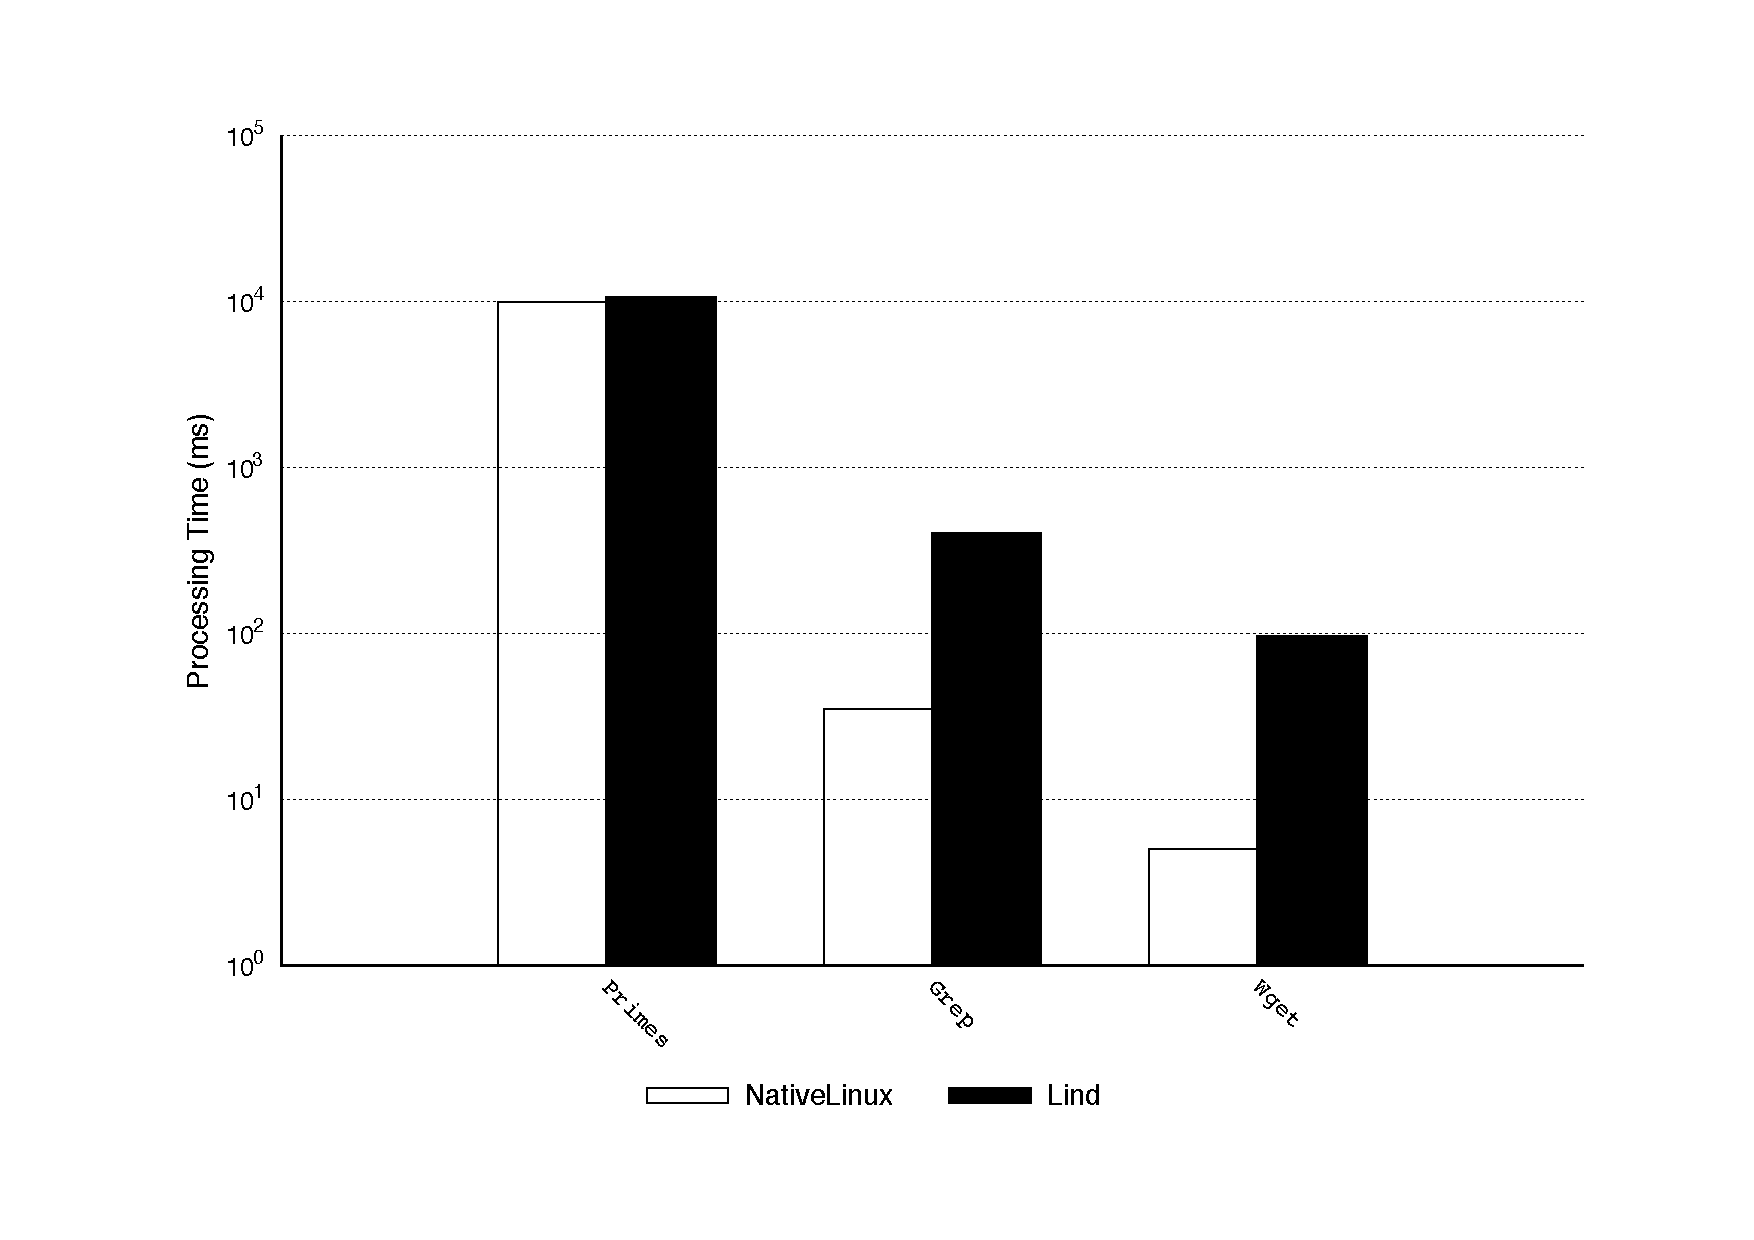
\includegraphics[width=1.0\columnwidth]{diagram/lind_oakland16_performance.pdf}
\caption{Application Runtime Performance: Native Linux vs. Lind}
\label{fig:performance_applications}
\end{figure}

While efficiency was not our main goal, we also evaluated Lind to see
how its performance compared to other systems in a real-world application.
Note that we did not optimize the performance of Lind in any way.

We first compiled and ran three widely used applications:
a primes calculator, GNU \texttt{grep}, and GNU \texttt{wget}. All ran unaltered and
correctly inside Lind. The source code of each of the applications remained
unmodified. To run the applications, it was sufficient to just recompile the
source code using NaCl's compiler and Lind's \texttt{glibc} to call
into SafePOSIX.
Figure \ref{fig:performance_applications} shows the runtime performance
results.
The primes application run in Lind has a 6\% performance overhead compared to
Native Linux. CPU bound applications, like the primes, engender little overhead,
because they run only inside the NaCl computation sandbox. No system calls are required,
and there is no need to go through the safe POSIX interface. The small amount of overhead
is generated by NaCl's instruction alignment at building time. Another reason for the overhead
is that the instructions built by NaCl have a higher rate of cache misses, which can slowdown the
program.
We expect other CPU bound processes to behave similarly.
\texttt{grep} experienced roughly 11x slowdown over Native Linux, while \texttt{wget}
slowdown was roughly 19x. Since they are both I/O heavy applications,
each repeatedly calls into the SafePOSIX code which then reimplements
the call.  The additional computation of SafePOSIX produced the additional
overhead.

Next, we ran the Tor router software in Lind \cappos{what version}. Tor simply
needs to be recompiled to run in Lind.
We used the benchmarks that come with Tor to test its common operations.
A summary of the results is shown in Table \ref{table:performance_tor}. The
benchmarks focus on cryptographic operations,
which are CPU intensive, but also make system calls like \texttt{getpid}, and reads to
\texttt{/dev/urandom}.
The digest operations time the access of a map of message digests.
The AES operations time AES encryptions of several sizes and message
digest creation.
Cell processing executes full packet encryption and decryption. In our
test, Lind slowed down these operations by 2.5x to 5x. We believe these
slowdowns are due to the increased code size produced by NaCl,
\cappos{I'm not sure why this would be.  Does NaCl show this too?}
and the
increased overhead from Lind's safe POSIX system call interface.

As shown above,  Lind incurs some performance overhead in most cases.
It should be noted that, we have not  yet attempted to optimize its performance.
However, since an attack on the kernel has devastating
consequences, %at this initial stage,
a tradeoff between security and performance is well justified.
The fact that Lind is able to run many \cappos{4 applications isn't many...
Do we have Apache numbers or something else to quantify?} legacy applications
suggests that it
is a positive step towards building new secure systems.

\begin{table}
\centering
\scriptsize
\caption{Performance Results on Tor's Built-in Benchmark Program: Native
Linux vs. Lind.}
\begin{tabular}{|r|r|r|r|}
  \hline
  {\bf Benchmark} & {\bf Native Code} & {\bf Lind} & {\bf Impact}  \\
  \hline
  Digest Tests: & & & \\
  Set & 54.80 nsec/element & 176.86 nsec/element & 3.22x \\
  Get & 42.30 nsec/element & 134.38 nsec/element & 3.17x \\
  Add & 11.69 nsec/element & 53.91 nsec/element & 4.61x \\
  IsIn & 8.24 nsec/element & 39.82 nsec/element & 4.83x \\
  \hline
  AES Tests: & & & \\
  1 Byte & 14.83 nsec/B & 36.93 nsec/B & 2.49x \\
  16 Byte & 7.45 nsec/B & 16.95 nsec/B & 2.28x \\
  1024 Byte & 6.91 nsec/B & 15.42 nsec/B & 2.23x \\
  4096 Byte & 6.96 nsec/B & 15.35 nsec/B & 2.21x \\
  8192 Byte & 6.94 nsec/B & 15.47 nsec/B & 2.23x \\
  Cell Sized & 6.81 nsec/B & 14.71 nsec/B & 2.16x \\
  \hline
  Cell Processing: & & & \\
  Inbound & 3378.18 nsec/cell & 8418.03 nsec/cell & 2.49x \\
  (per Byte) & 6.64 nsec/B & 16.54 nsec/B & - \\
  Outbound & 3384.01 nsec/cell & 8127.42 nsec/cell & 2.40x \\
  (per Byte) & 6.65 nsec/B & 15.97 nsec/B & - \\
  \hline
\end{tabular}
\label{table:performance_tor}
\end{table}
